\subsubsection{Biblioteca Multimedia Simple y R\'apida (Simple amd Fast Multimedia Library, SFML)}
    Para el desarrollo de nuestro Trabajo Terminal (TT), se utiliz\'o la Biblioteca Multimedia Simple y R\'apida (Simple amd Fast Multimedia Library, SFML), 
        la cual es una biblioteca gr\'afica multiplataforma de c\'odigo abierto, que proporciona una Interfaz de Programaci\'on de Aplicaciones (Application Programming Interface, API) simple y f\'acil de usar 
        para el desarrollo de aplicaciones multimedia y videojuegos. SFML est\'a escrita en C++ y proporciona una interfaz de 
        programaci\'on orientada a objetos, que facilita la creaci\'on de aplicaciones gr\'aficas y multimedia de alto rendimiento.
    \vskip 0.5cm
    En nuestro caso lo estamos usando en C++, ya que buscamos un mejor rendimiento en tiempo de ejecuci\'on la comparaci\'on la podemos ver
        en la Figura \ref{fig:tiempoEjecucion}. Adem\'as de que SFML es una biblioteca muy popular en la comunidad de desarrollo de videojuegos, por lo que es una buena opci\'on 
        para el desarrollo de nuestro simulador. Y no es tan complicada como Vulkan o DirectX, y ya que el prop\'osito de nuestro trabajo 
        no es el desarrollo del simulador sino del Robot, no lo consideramos vital el uso de una biblioteca m\'as compleja.
    \vskip 0.5cm
    % Parrafo 3
    SFML proporciona una serie de m\'odulos que permiten el desarrollo de aplicaciones multimedia y videojuegos, 
        incluyendo gr\'aficos 2D, sonido, entrada de teclado y rat\'on, y redes. Adem\'as, SFML proporciona una serie de 
        clases y funciones que facilitan la creaci\'on de aplicaciones gr\'aficas y multimedia, como ventanas, sprites, 
        texturas, fuentes, sonidos, y eventos. SFML tambi\'en proporciona una serie de m\'odulos que permiten la creaci\'on 
        de aplicaciones multimedia y videojuegos, como gr\'aficos 2D, sonido, entrada de teclado y rat\'on, y redes.
    \vskip 0.5cm
    % Parrafo 4
    SFML es una biblioteca multiplataforma que est\'a disponible para Windows, Linux y macOS, y es compatible con una 
        amplia variedad de compiladores y entornos de desarrollo, como Visual Studio, Code::Blocks, y Xcode. SFML tambi\'en 
        proporciona una serie de m\'odulos que permiten la creaci\'on de aplicaciones multimedia y videojuegos, como gr\'aficos 
        2D, sonido, entrada de teclado y rat\'on, y redes.
    \vskip 0.5cm
    % Parrafo 5
    SFML es una biblioteca de c\'odigo abierto que est\'a disponible bajo la licencia zlib/png, lo que significa que 
        se puede utilizar de forma gratuita en proyectos comerciales y no comerciales, y se puede modificar y distribuir 
        libremente. SFML tambi\'en proporciona una serie de m\'odulos que permiten la creaci\'on de aplicaciones multimedia 
        y videojuegos, como gr\'aficos 2D, sonido, entrada de teclado y rat\'on, y redes.
    \vskip 0.5cm
    \begin{figure}[h]  
        \centering
        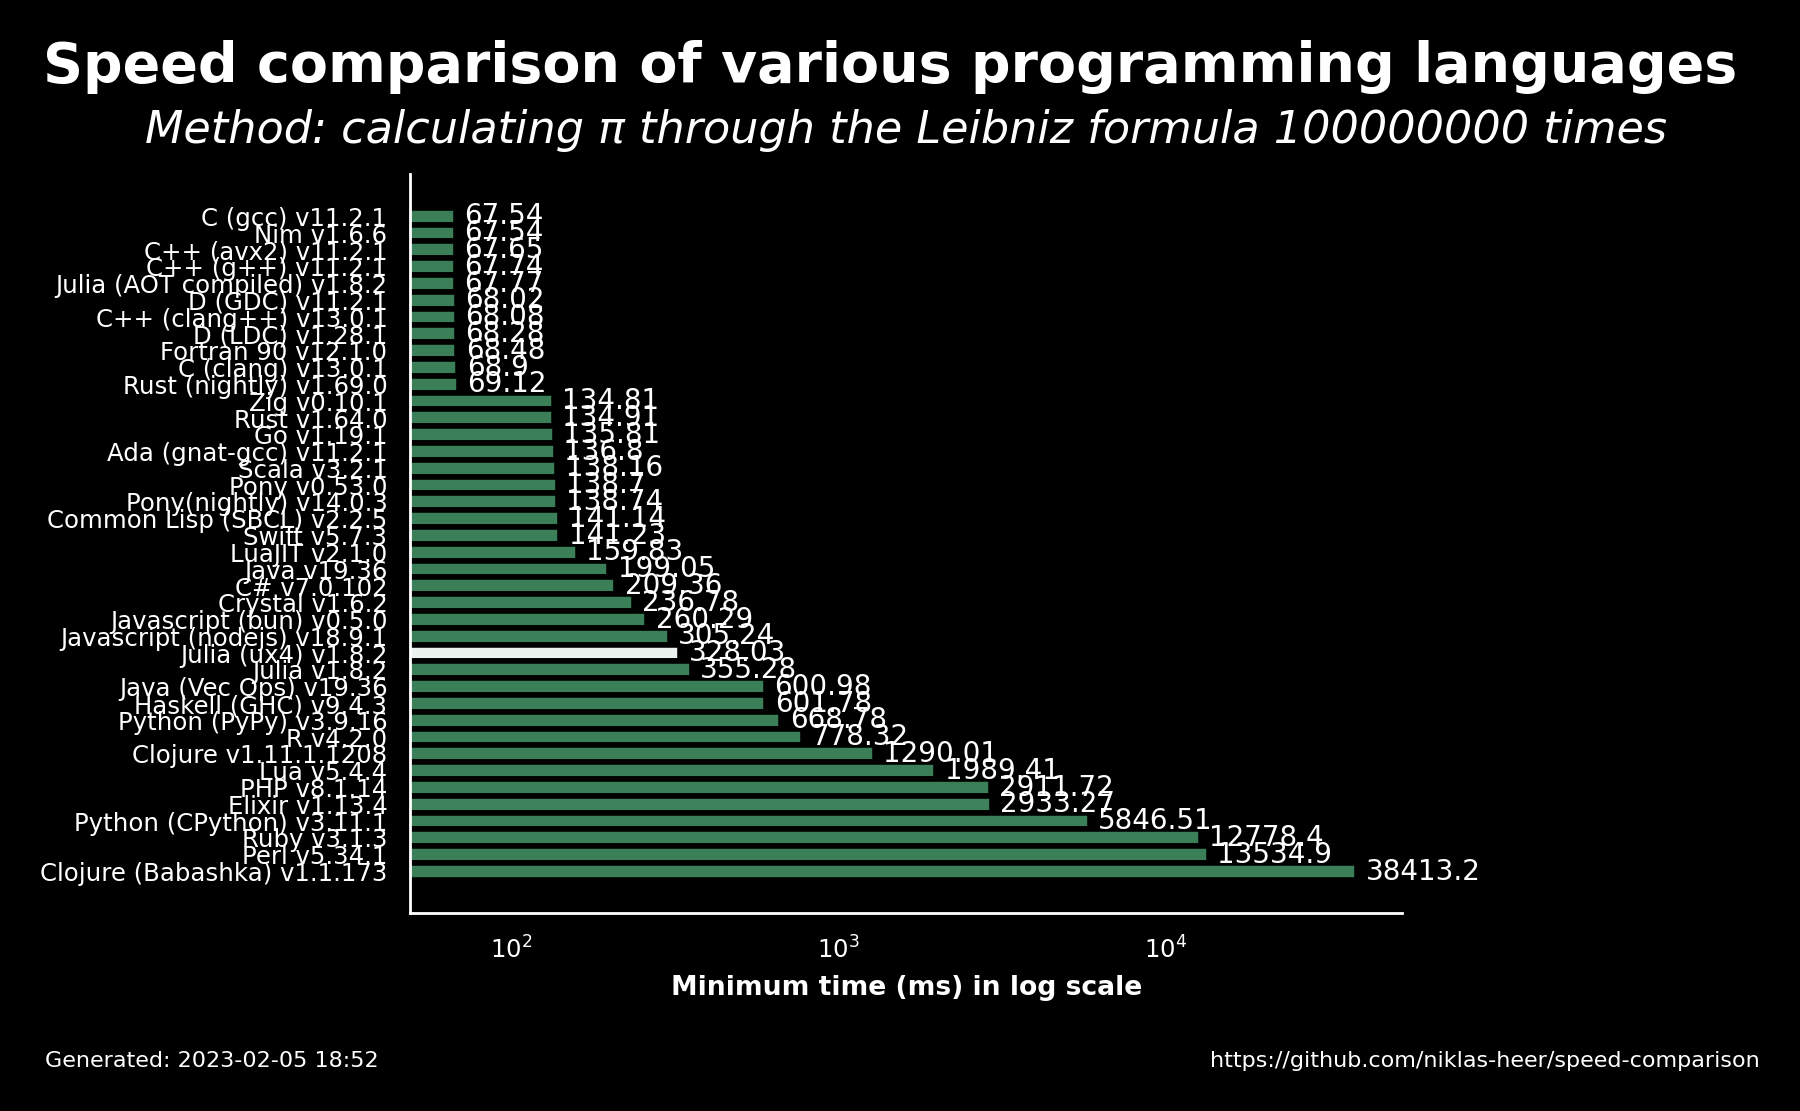
\includegraphics[width=0.5\textwidth]{./images/marco_teorico/Grafico/ComparacionLenguajes.png}
        \caption{Comparaci\'on de tiempo de ejecuci\'on entre diferentes lenguajes de Programaci\'on. Esta gr\'afica fue generada Heer \cite{ComparitionLanguajes}}
        \label{fig:tiempoEjecucion}
    \end{figure}
    \clearpage